% This is "sig-alternate.tex" V2.0 May 2012
% This file should be compiled with V2.5 of "sig-alternate.cls" May 2012
%
% This example file demonstrates the use of the 'sig-alternate.cls'
% V2.5 LaTeX2e document class file. It is for those submitting
% articles to ACM Conference Proceedings WHO DO NOT WISH TO
% STRICTLY ADHERE TO THE SIGS (PUBS-BOARD-ENDORSED) STYLE.
% The 'sig-alternate.cls' file will produce a similar-looking,
% albeit, 'tighter' paper resulting in, invariably, fewer pages.
%
% ----------------------------------------------------------------------------------------------------------------
% This .tex file (and associated .cls V2.5) produces:
%       1) The Permission Statement
%       2) The Conference (location) Info information
%       3) The Copyright Line with ACM data
%       4) NO page numbers
%
% as against the acm_proc_article-sp.cls file which
% DOES NOT produce 1) thru' 3) above.
%
% Using 'sig-alternate.cls' you have control, however, from within
% the source .tex file, over both the CopyrightYear
% (defaulted to 200X) and the ACM Copyright Data
% (defaulted to X-XXXXX-XX-X/XX/XX).
% e.g.
% \CopyrightYear{2007} will cause 2007 to appear in the copyright line.
% \crdata{0-12345-67-8/90/12} will cause 0-12345-67-8/90/12 to appear in the copyright line.
%
% ---------------------------------------------------------------------------------------------------------------
% This .tex source is an example which *does* use
% the .bib file (from which the .bbl file % is produced).
% REMEMBER HOWEVER: After having produced the .bbl file,
% and prior to final submission, you *NEED* to 'insert'
% your .bbl file into your source .tex file so as to provide
% ONE 'self-contained' source file.
%
%
% For tracking purposes - this is V2.0 - May 2012

\documentclass{sig-alternate}
\usepackage{color}
\usepackage[colorlinks,citecolor=blue]{hyperref}

\begin{document}

\conferenceinfo{Web Science}{2015 DIKU, Denmark}
\title{WS 2015 Project 1:\\Web Size}
\numberofauthors{1} 
\author{
\alignauthor 
Anonymous
}
\maketitle



\section{Introduction}
The internet has grown exponentialy since Lawrence and Gile's paper on estimating the size of the Web. Their research has evolved into different types of methods that are currently used to measure the coverage of the major World Wide Web search engines. Estimating the size of the whole Web is quite difficult, due to its dynamic nature. In 1998, Lawrence and Giles [6, 3] gave a lower bound 800 million pages. These estimates are now obsolete.\\

The methodology that Gulli and Signorini used to conduct a new measurement of the size of the web is very similar to Lawrence and Giles approach. Their approach was based on analyzing the top 3 search engines from 2005: Google (which has the largest number of indexed pages of any search engine), Yahoo!, Ask/Teoma and MSM. From their findings, Google indexed around 68.2\% of any other search engine, MSN indexed around 49.2\%, Ask/Teoma index around 43.5\% and Yahoo! index about 59.1\%. Averaging their values, they estimated the Indexable Web to be approximately 11.5 billion pages. As reported in their paper, the estimated intersection of all four indexes is 28.85\%, or about 2.7 billion pages, and their union is about 9.36 billion pages. \\

Another way of crawling the web in search was presented by Brian and Alvin Moore in the "Sizing the Internet" paper published in 2000. Their study was done by using the Cyveillence proprietary technology (NetSapien Technology). Their approach was by analysing 350 million links and crawling each page for other distinct URLs[]. The model analyzes spesific data associated with the links. The study ran over a four month period. By continuously referencing pages and exmining the links, the model is able to track the frequency with which unique URLs are encountered, both for the first time and each time thereafter. Their finding had surpassed their expectations with the number of unique pages on the Internet of 2.1 billion, and number of unique pages added per day of 7.3 million.\\


\section{Methodology}

The methodology I used for estimating the size of the web is very similar to Giles and Lawrence's approach from 1998. For crawling the web I used 500 queries and 3 search engines. The search engines that were considered for this experiment are: Bing, Baidu and Yandex. I have used these ones because Google, Yahoo! and other bigger search engines have protection mechanisms that prevent artificil polling of search results. If the crawler request to many searches in a short amount of time, Google enforces a cooldown period for additional queries. In 2014, Bing reports that it has indexed more than 17 billion pages [https://www.ventureharbour.com/visualising-size-google-bing-yahoo/s]. Baidu has indexed over 740 million web pages, 80 million images, and 10 million multimedia files. [ "MSN Money – BIDU". MSN Money. Archived from the original on May 1, 2006. Retrieved 2006-05-11.]. Yandex has around 15 billion indexed pages[Project description].\\

The software that I used for crawling these search engines is GoogleScraper[https://github.com/NikolaiT/GoogleScraper](A Python module to scrape several search engines (like Google, Yandex, Bing, Duckduckgo, Baidu and others) by using proxies (socks4/5, http proxy) and with many different IP's, including asynchronous networking support). It worked decent enough for carrying out this assignment and it has some extra features that helped improve performance during crawling (for example multi-threding support). The experiment was carried out in a time span of 2 days of non-stop crawling and data gathering.\\ 

\subsection{Crawling Particularities}

For each of the 500 queries I retrieve 20 pages of results. Twenty pages seemd sufficient for retrieving relative search results, because search engines often retrive similar results for queries and not the actual query term. Each page contains between 10-15 results. GoogleScraper scrapes the three search engines in the same time with 10 worker threads. GoogleScrapes saves the URLs in the google\_scraper.db SQL database. After finishing all 30000 keywords we begin analyzing the newly created database of links, references, search terms and serach engines to make an estimation on how big is the Web.\\

To create a realistic estimate of the size of the Web, based on the current parameters, we would be checking the unique links retrived by the crawler. Some links are redirects to different pages (for example www.baidu.com/safiahsiohasda4124124) we will leave them out of the data analysis because we don not know if the links would take us to the same pages that other search engines have retrieved for us. Also, because we are comparing links relative to actual documents we do not know if the pages contain the same information themselves. This will have an impact on the estimate of our web size. In 'Searching the world wide web' they state that they download each page and check that the query term occurs in the document. This is a very high computational task and we would require different hardware in order to obtain the same results.\\

Unfortunately after crawling for two days, I realised that bing and baidu have autocorrection by default and they would retrive the same results for two different queries. For example the queries "apple" and "aple" will retun the same search results. This omission greatly impacts our search results.\\

\section{Findings}
Report your findings in tables and figures (equivalent to Tables 1-2 and Figures 1-3 in \cite{LawLee1998}). You must also discuss these tables and figures.


\section{Conclusions}
Describe your conclusions. 

\begin{table}
\centering
\caption{Toy table. Use this as a template for making your own tables.}
\begin{tabular}{|c|c|l|} \hline
Non-English or Math&Frequency&Comments\\ \hline
\O & 1 in 1,000& For Swedish names\\ \hline
$\pi$ & 1 in 5& Common in math\\ \hline
\$ & 4 in 5 & Used in business\\ \hline
$\Psi^2_1$ & 1 in 40,000& Unexplained usage\\
\hline\end{tabular}
\end{table}

\begin{figure}
\centering
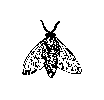
\epsfig{file=fly.eps}
\caption{Toy figure. Use this as a template for making your own figures.}
\end{figure}

% The following two commands are all you need in the
% initial runs of your .tex file to
% produce the bibliography for the citations in your paper.
\bibliographystyle{abbrv}
\bibliography{citations}  % sigproc.bib is the name of the Bibliography in this case
% You must have a proper ".bib" file
%  and remember to run:
% latex bibtex latex latex
% to resolve all references
%
% ACM needs 'a single self-contained file'!
%
%APPENDICES are optional
%\balancecolumns
%\appendix
%Appendix A
%\balancecolumns % GM June 2007
% That's all folks!
\end{document}
